\documentclass[aspectratio=169]{beamer}
\usepackage[utf8]{inputenc}
\usepackage{hyperref}
\usepackage{amsmath,amsfonts,amsthm,bm}
\usepackage{color}
\usepackage{graphicx} % Allows including images
\usepackage{subcaption}
\usepackage{booktabs} % Allows the use of \toprule, \midrule and \bottomrule in tables
\usepackage{tikz}
%\usepackage{pgfplots}
\usepackage{listings}
\usepackage{courier}
\usepackage[version=4]{mhchem}
\usepackage{array}

\lstset{ %
    basicstyle=\scriptsize\ttfamily, % fonts that are used for the code
    breakatwhitespace=false,         % sets if automatic breaks should only happen at whitespace
%breaklines=true,                 % sets automatic line breaking
%captionpos=b,                    % sets the caption-position to bottom
    commentstyle=\color{gray}\textit,    % comment style
    keepspaces=true,                 % keeps spaces in text, useful for keeping indentation of code (possibly needs columns=flexible)
    keywordstyle=\color{blue},       % keyword style
    language=Python,                 % the language of the code
%otherkeywords={*,...},          % if you want to add more keywords to the set
    rulecolor=\color{black},         % if not set, the frame-color may be changed on line-breaks within not-black text (e.g. comments (green here))
    showspaces=false,                % show spaces everywhere adding particular underscores; it overrides 'showstringspaces'
    showstringspaces=false,          % underline spaces within strings only
    showtabs=false,                  % show tabs within strings adding particular underscores
    stringstyle=\color{red}, % string literal style
    tabsize=4,                       % sets default tabsize to 2 spaces
    columns=fixed                    % Using fixed column width (for e.g. nice alignment)
}

\hypersetup{
    colorlinks=true,
    linkcolor=red,
    filecolor=magenta,
    urlcolor=red,
}

\DeclareMathOperator*{\argmax}{argmax}
\DeclareMathOperator*{\argmin}{argmin}
\let \vec \mathbf

\newcommand{\classname}{NANO266}
\newcommand{\classyear}{Fall 2024}
\mode<presentation> {
    \usetheme{CambridgeUS}
    \setbeamertemplate{footline}[text line]{%
        \parbox{\linewidth}{\vspace*{-8pt}\classname\hfill\classyear\hfill\insertpagenumber}}

    %\setbeamertemplate{footline}[page number]
    \setbeamertemplate{navigation symbols}{}
}


\title[\classname Properties of Molecules from QM]{\classname~- Quantum Mechanical Modeling of Materials and Nanostructures\\Properties of Molecules from QM}

\author{Shyue Ping Ong}
\institute[UCSD]{University of California, San Diego\\
\medskip
}
\date{\classyear} % Date, can be changed to a custom date

\begin{document}


    \begin{frame}
        \titlepage % Print the title page as the first slide
    \end{frame}


    \begin{frame}{The World of Materials}

        \begin{table}[]
            \centering
            \begin{tabular}{p{2cm}|p{3cm}|p{4cm}|p{3cm}}
                & Molecules                                  & Liquids/amorphous/etc.    & Crystals                \\
                \hline
                \hline
                Modelled as & Isolated gas phase                         & Challenging for direct QM & Periodic infinite solid \\
                Basis set   & Localized basis functions, e.g., Gaussians & Simplified models         & Plane waves
            \end{tabular}
        \end{table}
    \end{frame}

    \begin{frame}{Overview}
        In this lecture, we will:
        \begin{itemize}
            \item survey the study of properties of isolated molecules using quantum mechanical approaches.
            \item connect calculations with real world properties.
            \item discuss performance and accuracy.
        \end{itemize}

        Lab 1: Study of ammonia formation using QM

    \end{frame}


    \begin{frame}{Things you get from QM calculations}
        Energies - Already covered in previous lectures\newline
        \newline
        Geometries\newline
        \newline
        Charge densities and spectroscopic properties\newline
        \newline
        And their derivatives…
    \end{frame}


    \begin{frame}{Thermodynamics Ensembles}

        QM gives the single molecule energies.\newline
        \newline
        Question: How do we get ensemble thermodynamic variables from single-molecule calculations?\newline
        \newline
        Answer: Statistical mechanics

    \end{frame}

    \begin{frame}{Recap: Statistical mechanics}

        Partition function

        \begin{equation*}
            Z(N, V, T) = \sum_{i} e^{-\beta E_i(N,V)}
        \end{equation*}

        where $i$ is the index of microstates, $\beta = 1/k_b T$ and $E_i$ is the energy.

        \begin{eqnarray*}
            U & = & k_B T^2 \left( \frac{\partial \ln Z} {\partial T} \right)_{N,V}\\
            H & = & U + PV\\
            S & = & k_B \ln Z + k_B \left( \frac{\partial \ln Z} {\partial T} \right)_{N,V}\\
            G & = & H - TS
        \end{eqnarray*}
    \end{frame}

    \begin{frame}{Assumption: Ideal gas molecules}
        Since ideal gas molecules do not interact,

        \begin{equation*}
            Z(N, V, T) = \frac{z(V,T)^N}{N!}
        \end{equation*}

        where $z$ is the molecular partition function.\newline
        \newline
        The molecular partition function can be further broken down into separable electronic, translational, rotational, and vibrational components:

        \begin{equation*}
            z(V,T) = z_{elec}(T)z_{trans}(V, T)z_{rot}(T)z_{vib}(T)
        \end{equation*}

        Combining the results and taking the natural log, we have:


        \begin{equation*}
            \ln Z(N, V, T) = N[z_{elec}(T)+z_{trans}(V, T)+z_{rot}(T)+z_{vib}(T)]-N\ln N + N
        \end{equation*}

    \end{frame}

    \begin{frame}{Electronic and Translation Partition Function}
        \textbf{Electronic}
        \begin{itemize}
            \item Typically, excited states are much higher in energy and make no significant contribution to partition function below a few 1000K $\implies$ Just the electronic energy from QM.
            \item If there is a non-singlet ground state, there are contributions to the electronic entropy.
        \end{itemize}

        \textbf{Translational (Particle in box)}

        \begin{eqnarray*}
            z_{trans}(V, T) & = & \left( \frac{2\pi Mk_BT}{h^2} \right)^{\frac{3}{2}} V\\
            U_{trans} & = & \frac{3}{2} RT\\
            S_{trans}^0 & = & R\left \{ \ln \left [{\left( \frac{2\pi Mk_BT}{h^2} \right) ^{\frac{3}{2}}}  \frac{V}{N_A} \right ] + \frac{5}{2} \right  \}
        \end{eqnarray*}

    \end{frame}


    \begin{frame}{Vibrational frequencies and energies}

        Based on quantum mechanical harmonic oscillator assumption (3N – 6 degrees of freedom)

        \begin{equation*}
            E = (n+\frac{1}{2})h\omega,  \omega = \frac{1}{2\pi}\sqrt{\frac{k}{\mu}}
        \end{equation*}
        where $k$ are the force constants and $\mu$ is the reduced mass.\newline
        \newline
        To obtain the force constants, one simply needs to calculate the 2nd derivative of the energy with respect to bond stretching at equilibrium bond geometry.\newline
        \newline
        Can be done analytically for HF, MP2, DFT, CISD, CCSD.

    \end{frame}

    \begin{frame}{Vibrational Partition Function}
        \begin{columns}
            \column{0.7\textwidth}

            \begin{eqnarray*}
                z_{vib}(T) & = & \frac{1}{1-e^{-\frac{h\omega}{k_BT}}}\\
                U_{vib} & = & \prod_{i=1}^{3N-6} \frac{1}{1-e^{-\frac{h\omega_i}{k_BT}}}\\
                S_{vib}^0 & = & R \sum_{i=1}^{3N-6} \left [ \frac{h\omega_i}{k_BT(e^{\frac{h\omega_i}{k_BT}}-1)} - \ln (1-e^{-\frac{h\omega_i}{k_BT}}) \right ]
            \end{eqnarray*}

            Scaling factors applied to account for systematic errors, e.g., force constants in HF are too large.

            \column{0.3\textwidth}

            \begin{figure}
                \centering
                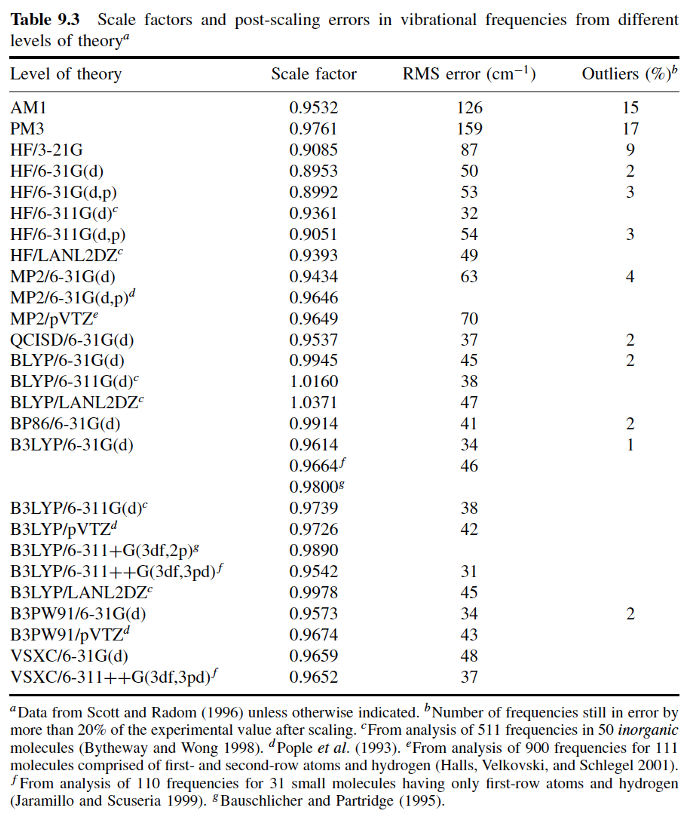
\includegraphics[width=\linewidth]{lectures/figures/4_scaling_factors.png}
            \end{figure}
        \end{columns}

    \end{frame}

    \begin{frame}{Rotational Partition Function}

        Different treatments for linear and non-linear molecules to be treated separately.

        Refer to statistical mechanics textbook.

    \end{frame}


    \begin{frame}{Typical Free energy Calculation Procedure}

        \begin{figure}
            \centering
            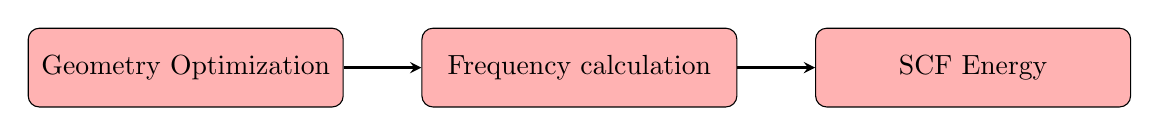
\begin{tikzpicture}[node distance=5cm]
                \tikzstyle{roundrect} = [rectangle, rounded corners, minimum width=4cm, minimum height=1cm,text centered, draw=black, fill=red!30]
                \tikzstyle{arrow} = [thick,->,>=stealth]
                \node (go) [roundrect] {Geometry Optimization};
                \node (freq) [roundrect, right of=go] {Frequency calculation
                };
                \node (scf) [roundrect, right of=freq] {SCF Energy};

                \draw [arrow] (go) -- (freq);
                \draw [arrow] (freq) -- (scf);
            \end{tikzpicture}
        \end{figure}
        \begin{itemize}
            \item Geometry optimization (GO) typically at a lower level of theory and smaller basis set.
            \item Frequency calculation performed at the same level of theory as GO.
            \item SCF energy calculation performed at higher level of theory and bigger basis set.
        \end{itemize}

    \end{frame}


    \begin{frame}{Selecting model chemistries}
        \begin{columns}
            \column{0.5\textwidth}
            \begin{figure}
                \centering
                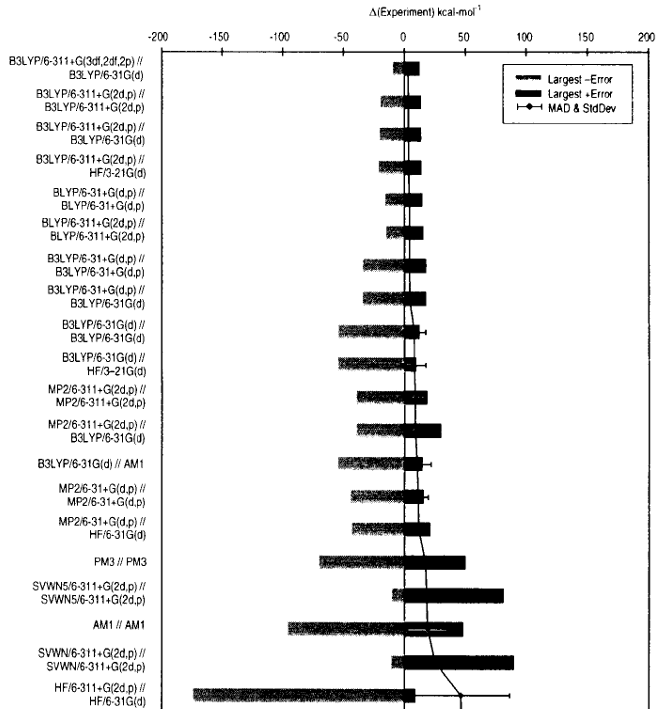
\includegraphics[width=0.45\linewidth]{lectures/figures/4_model_chem.png}
            \end{figure}
            \column{0.5\textwidth}
            Adapted from \cite{foresmanExploringChemistryElectronic1996}.

            \begin{alertblock}{Bottom line}
                Cheap functional + small basis set for relaxation followed by accurate functional + large basis set for SCF energy works well.

            \end{alertblock}

        \end{columns}

    \end{frame}

    \begin{frame}{Practical reaction calculations}

        Reaction 1: Only involves gas phases.\newline
        \newline
        \ce{N2(g) + H2(g) -> 2NH3(g)}\newline
        \newline
        Reaction 2: Involves condensed as well as gas phases.\newline
        \newline
        \ce{C(s) + O2(g) -> CO2(g)}

    \end{frame}

    \begin{frame}{Thermodynamic cycle method}
        \begin{figure}
            \centering
            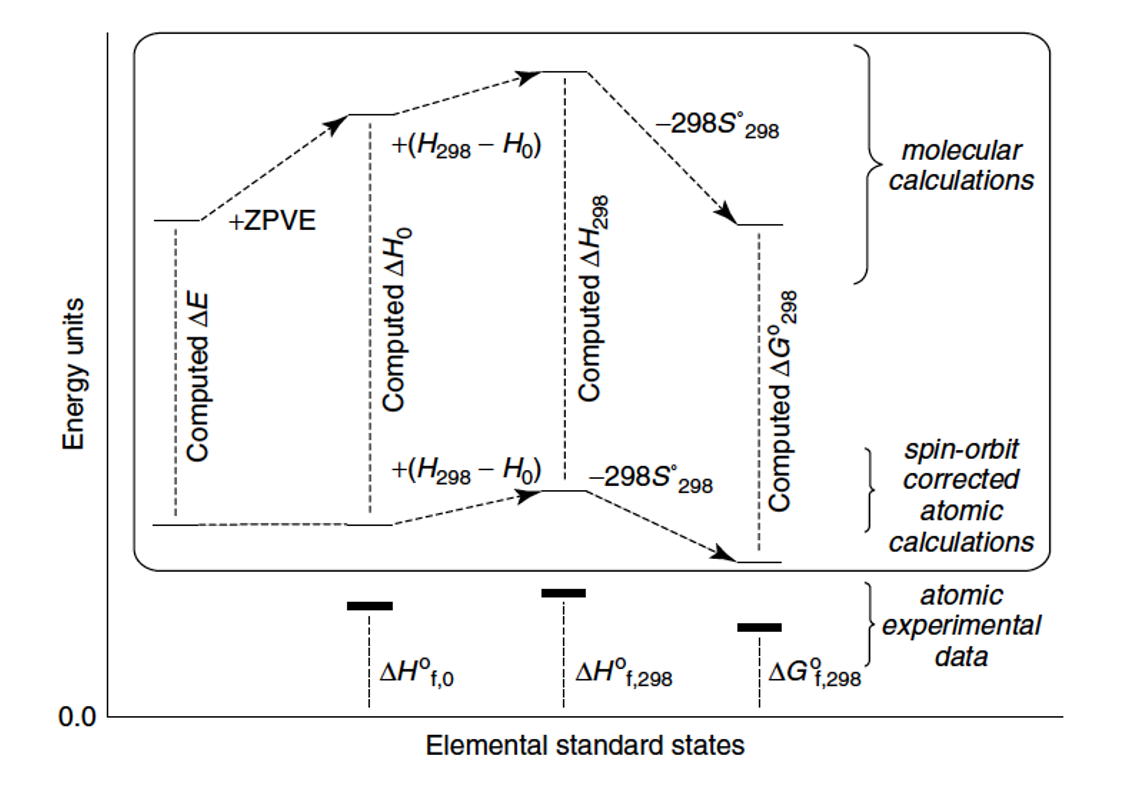
\includegraphics[width=0.4\linewidth]{lectures/figures/4_energy_diagram.png}
        \end{figure}
        \begin{eqnarray*}
            \Delta H_{f,298}^0(M) & = & E(M) + ZPE(M) + [H_{298}(M) - H_0(M)]\\
            && - \sum_z^{atoms} \{E(X_z)+[H_{298}(X_z) - H_0(X_z)]\} + \sum_z^{atoms}\Delta H_{f,298}^0(X_z)
        \end{eqnarray*}

    \end{frame}

    \begin{frame}{Ionization energies and electron affinities}
        \textbf{Koopman’s Theorem}: HOMO energy as estimate of vertical IE fairly reasonable due to canceling of basis set incompleteness and correlation errors in Hartree-Fock.\newline
        \newline
        \textbf{$\Delta$SCF}: Calculate energy of molecule in neutral and positively / negatively charged state,
        \begin{equation*}
            IE = E(\ce{M+}) - E(\ce{M})
        \end{equation*}

        Generally works well if diffuse functions are used to model ions with diffuse electron clouds.
    \end{frame}

    \begin{frame}{Atomic charges}
        \begin{itemize}
            \item Class II charges – determined by partitioning of wave functions (a somewhat arbitrary process).
            \item Mulliken approach – partition according to degree atomic orbitals contribute to wave function.
            \item Lowdin – Transform AO basis functions to orthonormal set.
            \item Natural population analysis (NPA) – Orthogonalization in four-step process to render electron density as compact as possible before Mulliken analysis.
        \end{itemize}

    \end{frame}

    \begin{frame}{NMR spectral properties}
        General recommendation is very large basis sets (at least triple-$\zeta$) and lots of diffuse and polarization functions.\newline
        \newline
        Not possible to predict chemical shift for nuclei of heavy atoms with effective core potentials.\newline
        \newline
        For molecules comprising first row atoms, heavy-atom chemical shifts can be obtained with a fair degree of accuracy even with HF (though MP2 and DFT fares much better).

    \end{frame}

    \begin{frame}[allowframebreaks]{Bibliography}
        \bibliographystyle{unsrt}
        \bibliography{refs}
    \end{frame}



    \begin{frame}
        \Huge{\centerline{The End}}
    \end{frame}

\end{document}

